\tikzset{every picture/.style={line width=0.75pt}} %set default line width to 0.75pt        

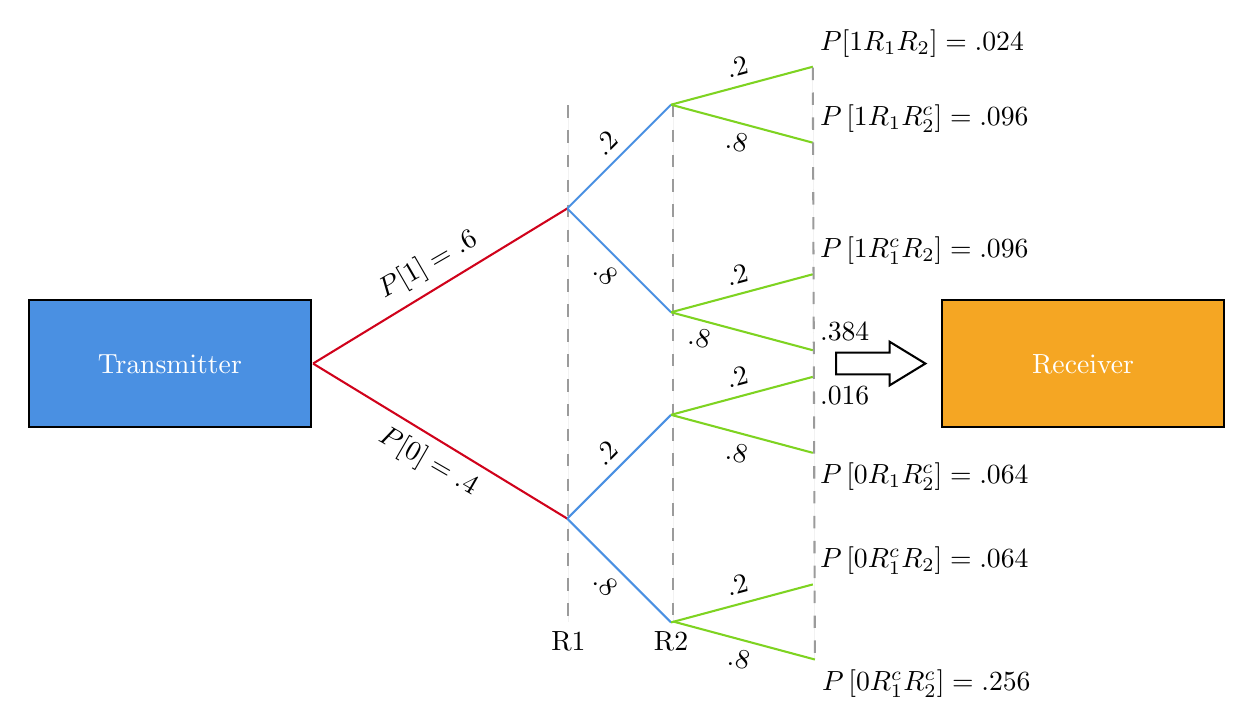
\begin{tikzpicture}[x=0.75pt,y=0.75pt,yscale=-1,xscale=1]
%uncomment if require: \path (0,375); %set diagram left start at 0, and has height of 375

%Straight Lines [id:da7733451095996544] 
\draw [color={rgb, 255:red, 208; green, 2; blue, 27 }  ,draw opacity=1 ]   (147,195.5) -- (269.47,270.21) ;
%Shape: Rectangle [id:dp6454339282474542] 
\draw  [fill={rgb, 255:red, 74; green, 144; blue, 226 }  ,fill opacity=1 ] (10,165) -- (146,165) -- (146,226) -- (10,226) -- cycle ;
%Straight Lines [id:da8481277726765063] 
\draw [color={rgb, 255:red, 155; green, 155; blue, 155 }  ,draw opacity=1 ][fill={rgb, 255:red, 155; green, 155; blue, 155 }  ,fill opacity=1 ] [dash pattern={on 4.5pt off 4.5pt}]  (270,71) -- (270,320) ;
%Straight Lines [id:da022158918268141536] 
\draw [color={rgb, 255:red, 208; green, 2; blue, 27 }  ,draw opacity=1 ]   (147,195.5) -- (269.47,120.79) ;
%Straight Lines [id:da7936419917799142] 
\draw [color={rgb, 255:red, 74; green, 144; blue, 226 }  ,draw opacity=1 ]   (269.47,270.21) -- (319.47,220.21) ;
%Straight Lines [id:da035414361338925726] 
\draw [color={rgb, 255:red, 74; green, 144; blue, 226 }  ,draw opacity=1 ]   (269.47,120.79) -- (319.47,170.79) ;
%Straight Lines [id:da6315531716142546] 
\draw [color={rgb, 255:red, 74; green, 144; blue, 226 }  ,draw opacity=1 ]   (269.47,270.21) -- (319.47,320.21) ;
%Straight Lines [id:da43044094613045636] 
\draw [color={rgb, 255:red, 74; green, 144; blue, 226 }  ,draw opacity=1 ]   (269.47,120.79) -- (319.47,70.79) ;
%Straight Lines [id:da3197820199985336] 
\draw [color={rgb, 255:red, 155; green, 155; blue, 155 }  ,draw opacity=1 ][fill={rgb, 255:red, 155; green, 155; blue, 155 }  ,fill opacity=1 ] [dash pattern={on 4.5pt off 4.5pt}]  (320.47,70.79) -- (320.47,319.79) ;
%Straight Lines [id:da3376346045191835] 
\draw [color={rgb, 255:red, 126; green, 211; blue, 33 }  ,draw opacity=1 ]   (319.47,70.79) -- (387.78,52.49) ;
%Straight Lines [id:da5341817002427772] 
\draw [color={rgb, 255:red, 126; green, 211; blue, 33 }  ,draw opacity=1 ]   (319.47,70.79) -- (387.78,89.09) ;
%Straight Lines [id:da9132861107764135] 
\draw [color={rgb, 255:red, 126; green, 211; blue, 33 }  ,draw opacity=1 ]   (319.47,170.79) -- (387.78,152.49) ;
%Straight Lines [id:da0948837605825038] 
\draw [color={rgb, 255:red, 126; green, 211; blue, 33 }  ,draw opacity=1 ]   (319.47,170.79) -- (387.78,189.09) ;
%Straight Lines [id:da5858203477238184] 
\draw [color={rgb, 255:red, 126; green, 211; blue, 33 }  ,draw opacity=1 ]   (319.47,220.21) -- (387.78,201.91) ;
%Straight Lines [id:da7551891548818732] 
\draw [color={rgb, 255:red, 126; green, 211; blue, 33 }  ,draw opacity=1 ]   (319.47,220.21) -- (387.78,238.51) ;
%Straight Lines [id:da9857178211203643] 
\draw [color={rgb, 255:red, 126; green, 211; blue, 33 }  ,draw opacity=1 ]   (319.47,320.21) -- (387.78,301.91) ;
%Straight Lines [id:da15601066335308467] 
\draw [color={rgb, 255:red, 126; green, 211; blue, 33 }  ,draw opacity=1 ]   (320.47,319.79) -- (388.78,338.09) ;
%Straight Lines [id:da8229205540347613] 
\draw [color={rgb, 255:red, 155; green, 155; blue, 155 }  ,draw opacity=1 ][fill={rgb, 255:red, 155; green, 155; blue, 155 }  ,fill opacity=1 ] [dash pattern={on 4.5pt off 4.5pt}]  (387.78,52.91) -- (388.78,338.09) ;
%Shape: Rectangle [id:dp08161365143596533] 
\draw  [fill={rgb, 255:red, 245; green, 166; blue, 35 }  ,fill opacity=1 ] (450,165) -- (586,165) -- (586,226) -- (450,226) -- cycle ;
%Right Arrow [id:dp6874336891615508] 
\draw   (399,190.25) -- (424.8,190.25) -- (424.8,185) -- (442,195.5) -- (424.8,206) -- (424.8,200.75) -- (399,200.75) -- cycle ;

% Text Node
\draw (78,195.5) node  [color={rgb, 255:red, 255; green, 255; blue, 255 }  ,opacity=1 ] [align=left] {Transmitter};
% Text Node
\draw (206.54,155.2) node [anchor=south] [inner sep=0.75pt]  [rotate=-330]  {$P[ 1] =.6$};
% Text Node
\draw (206.54,235.8) node [anchor=north] [inner sep=0.75pt]  [rotate=-30]  {$P[ 0] =.4$};
% Text Node
\draw (270,323) node [anchor=north] [inner sep=0.75pt]   [align=left] {R1};
% Text Node
\draw (292.07,93.39) node [anchor=south] [inner sep=0.75pt]  [rotate=-315]  {$.2$};
% Text Node
\draw (292.07,148.19) node [anchor=north] [inner sep=0.75pt]  [rotate=-45]  {$.8$};
% Text Node
\draw (292.07,297.61) node [anchor=north] [inner sep=0.75pt]  [rotate=-45]  {$.8$};
% Text Node
\draw (292.07,242.81) node [anchor=south] [inner sep=0.75pt]  [rotate=-315]  {$.2$};
% Text Node
\draw (319.47,323.21) node [anchor=north] [inner sep=0.75pt]   [align=left] {R2};
% Text Node
\draw (352.75,58.35) node [anchor=south] [inner sep=0.75pt]  [rotate=-345]  {$.2$};
% Text Node
\draw (352.75,83.22) node [anchor=north] [inner sep=0.75pt]  [rotate=-15]  {$.8$};
% Text Node
\draw (334.75,177.22) node [anchor=north] [inner sep=0.75pt]  [rotate=-15]  {$.8$};
% Text Node
\draw (352.75,232.65) node [anchor=north] [inner sep=0.75pt]  [rotate=-15]  {$.8$};
% Text Node
\draw (353.75,332.22) node [anchor=north] [inner sep=0.75pt]  [rotate=-15]  {$.8$};
% Text Node
\draw (352.75,158.35) node [anchor=south] [inner sep=0.75pt]  [rotate=-345]  {$.2$};
% Text Node
\draw (352.75,207.78) node [anchor=south] [inner sep=0.75pt]  [rotate=-345]  {$.2$};
% Text Node
\draw (352.75,307.78) node [anchor=south] [inner sep=0.75pt]  [rotate=-345]  {$.2$};
% Text Node
\draw (518,195.5) node  [color={rgb, 255:red, 255; green, 255; blue, 255 }  ,opacity=1 ] [align=left] {Receiver};
% Text Node
\draw (389.78,49.51) node [anchor=south west] [inner sep=0.75pt]    {$P[ 1R_{1} R_{2}] =.024$};
% Text Node
\draw (389.78,149.09) node [anchor=south west] [inner sep=0.75pt]    {$P\left[ 1R_{1}^{c} R_{2}\right] =.096$};
% Text Node
\draw (389.78,85.69) node [anchor=south west] [inner sep=0.75pt]    {$P\left[ 1R_{1} R_{2}^{c}\right] =.096$};
% Text Node
\draw (389.78,185.69) node [anchor=south west] [inner sep=0.75pt]    {$.384$};
% Text Node
\draw (389.78,205.31) node [anchor=north west][inner sep=0.75pt]    {$.016$};
% Text Node
\draw (389.78,241.91) node [anchor=north west][inner sep=0.75pt]    {$P\left[ 0R_{1} R_{2}^{c}\right] =.064$};
% Text Node
\draw (389.78,298.51) node [anchor=south west] [inner sep=0.75pt]    {$P\left[ 0R_{1}^{c} R_{2}\right] =.064$};
% Text Node
\draw (390.78,341.49) node [anchor=north west][inner sep=0.75pt]    {$P\left[ 0R_{1}^{c} R_{2}^{c}\right] =.256$};


\end{tikzpicture}
